\documentclass[onecolumn]{article}

% figures
\usepackage[dvips]{epsfig}

% fonts
\usepackage{times}

%%%%%%%%%%%%%%%%%%%%%%%%%%%%
%% US letter
%%%%%%%%%%%%%%%%%%%%%%%%%%%%
\textwidth 17cm
\textheight 23.8cm
\oddsidemargin -4.5mm
\evensidemargin -4.5mm
\topmargin -15mm

% biblio GJI
\bibliographystyle{abbrv}

\newcommand{\toall}[1]{\textbf{*** All: #1 ***}}
\newcommand{\tojeroen}[1]{\textbf{*** Jeroen: #1 ***}}
\newcommand{\tobrian}[1]{\textbf{*** Brian: #1 ***}}
\newcommand{\tovala}[1]{\textbf{*** Vala: #1 ***}}
\newcommand{\tovalabrian}[1]{\textbf{*** Vala \& Brian: #1 ***}}
\newcommand{\tovalaqinya}[1]{\textbf{*** Vala \& Qinya: #1 ***}}
\newcommand{\toqinya}[1]{\textbf{*** Qinya: #1 ***}}
\newcommand{\tomin}[1]{\textbf{*** Min: #1 ***}}
\newcommand{\toalessia}[1]{\textbf{*** Alessia: #1 ***}}
\newcommand{\todimitri}[1]{\textbf{*** Dimitri: #1 ***}}

\newcommand{\nexxi}{\mbox{\texttt{NEX\_XI}}}
\newcommand{\nexeta}{\mbox{\texttt{NEX\_ETA}}}
\newcommand{\nprocxi}{\mbox{\texttt{NPROC\_XI}}}
\newcommand{\nproceta}{\mbox{\texttt{NPROC\_ETA}}}
\newcommand{\nchunks}{\mbox{\texttt{NCHUNKS}}}

\title{
\textbf{\Huge{SPECFEM3D\_GLOBE V3.6}} \\
\vspace{1.0cm}
User's Manual \\
%\vspace{1.0cm}
%\centerline{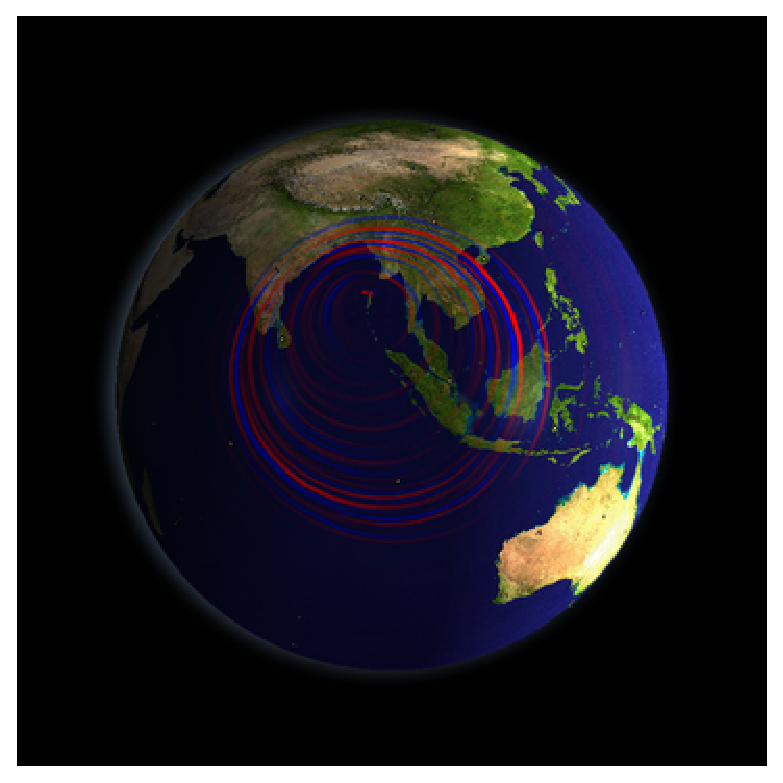
\includegraphics[width=0.75\textwidth]{figures/sumatra.eps}}
%\vspace{1.0cm}
%\centerline{
\includegraphics[angle=270,width=0.15\textwidth]{figures/seismo_lab_logo.eps}}
}

\begin{document}

\maketitle

\newpage

\tableofcontents

\newpage

\section{Introduction}

The software package SPECFEM3D\_GLOBE simulates global and regional
seismic wave propagation based upon the spectral-element method.
Effects due to lateral variations in compressional-wave speed,
shear-wave speed, density, a 3-D crustal model, ellipticity,
topography and bathymetry, the oceans, rotation, and
self-gravitation are all included.
The package can accommodate full 21-parameter anisotropy as well as
lateral variations in attenuation.
The latest additions involve adjoint capabilities and finite-frequency
kernel simulations.
For a detailed introduction to the spectral-element method as applied
to global and regional seismic wave propagation, please consult
\cite{KoTr02a,KoTr02b,KoRiTr02}.
If you use 3D mantle model S20RTS, please cite \cite{RiVaWo99}.

All SPECFEM3D\_GLOBE software is written in Fortran90, and conforms strictly to
the Fortran95 standard. It uses no obsolete features of Fortran77.
The package uses parallel programming based upon the
Message Passing Interface (MPI) \cite{GrLuSk94,Pac97}.

\section{Getting Started}
\label{section:gettingstarted}

The SPECFEM3D\_GLOBE software package comes in a gzipped tar ball.
In the directory in which you want to install the package type
`\texttt{tar -z -xvf SPECFEM3D\_GLOBE\_V3.6.tar.gz}'.
The directory \texttt{SPECFEM3D\_GLOBE\_V3.6} contains the source code.
To get started, you will be editing the \texttt{Makefile},
\texttt{constants.h}, and \texttt{precision.h} files in this
directory.

Our first objective is to be able to compile the software, which involves
setting the appropriate compiler flags in the \texttt{Makefile}.
The following flags need to be set for the compiler on your system:
\begin{description}
\item[\texttt{F90}] Path to the Fortran90 compiler.
\item[\texttt{MPIF90}] Path to MPI Fortran90.
\item[\texttt{MPI\_FLAGS}] Some systems require this flag to link to MPI libraries.
\item[\texttt{FLAGS\_CHECK}] Compiler flag for debugging code.
\item[\texttt{FLAGS\_NO\_CHECK}] Compiler flag for creating fast,
production-run code.
\end{description}
The \texttt{Makefile} contains a number of suggested entries for various compilers,
e.g., Portland, Intel, Absoft, NAG, and Lahey.
The software has run on a
wide variety of compute platforms, e.g., various PC clusters and machines from
Sun, SGI, IBM, Compaq, and NEC.
Select the compiler you wish to use on your system and choose the
related optimization flags. Note that the default flags in the
\texttt{Makefile} are undoubtedly not optimal for your system, so we
encourage you to experiment with these flags and to solicit advice from
your systems administrator. Selecting the right compiler
and compiler flags can make a tremendous
difference in terms of performance.
We find that, in general, the Intel and Portland
compilers produce the fastest code.
We welcome feedback on your experience with various compilers and flags.

Now that you have set the compiler information, you need to select a
number of flags in the \texttt{constants.h} file depending on your
system:
\begin{description}
\item[\texttt{FIX\_UNDERFLOW\_PROBLEM}] Set to \texttt{.true.} to fix
underflow trapping on some machines, e.g., most PC clusters.
This flag initializes the wavefield with a very small, but non-zero,
value to avoid underflow, i.e., `hanging' of the code as it is
multiplying zeros.
\item[\texttt{LOCAL\_PATH\_IS\_ALSO\_GLOBAL}] Set to
\texttt{.false.} on most cluster applications.
For reasons of speed,
the (parallel) mesher typically writes a (parallel) database for
the solver on the local disks of the compute nodes.
Some systems have no local disks, e.g., BlueGene or the Earth Simulator,
and other systems have a fast parallel file system, in which case
this flag should be set to \texttt{.true.}.
\end{description}
The package can run both in single and in double precision.
We typically run in single precision mode because this requires less
memory and is frequently faster. Select your preference
by selecting the appropriate setting in the \texttt{constants.h} file:
\begin{description}
\item[\texttt{CUSTOM\_REAL}] Set to \texttt{SIZE\_REAL} for single
precision and \texttt{SIZE\_DOUBLE} for double precision.
\end{description}
In the \texttt{precision.h} file:
\begin{description}
\item[\texttt{CUSTOM\_MPI\_TYPE}] Set to \texttt{MPI\_REAL} for single
precision and \texttt{MPI\_DOUBLE\_PRECISION} for double precision.
\end{description}
On a new system it is definitely worth experimenting with single versus
double precision simulations to determine which is faster.

When running on an SGI add "\texttt{setenv TRAP\_FPE OFF}"
to your .cshrc file \textit{before} compiling in order to
turn underflow trapping off.
When running on an IBM, e.g., an SP or a Power4, one needs to change
all the filename extensions from \texttt{*.f90} to \texttt{*.f}; a script is provided
in \texttt{DATA/util/change\_names\_IBM} to do that.
One also needs to change all the `\texttt{.f90}' extensions in the
\texttt{Makefile} to `\texttt{.f}'.

Finally, before compiling make sure that the
subdirectories \texttt{obj} and \texttt{OUTPUT\_FILES} exist within the directory
with the source code (\texttt{SPECFEM3D\_GLOBE\_V3.6}).
The \texttt{go\_mesher} script discussed below automatically takes
care of creating the \texttt{OUTPUT\_FILES} directory.

\section{Running the Mesher \texttt{xmeshfem3D}}
\label{section:mesher}

You are now ready to compile the mesher: in the
directory with the source code type `\texttt{make meshfem3D}'.
If all paths and flags have been set correctly, the mesher should now
compile and produce the executable \texttt{xmeshfem3D}.

Input for the mesher (and the solver)
is provided through the parameter file \texttt{Par\_file},
which resides in the subdirectory \texttt{DATA}.
Before running the mesher, a number of parameters need to be
set in the \texttt{Par\_file}. This requires a basic understanding
of how the spectral-element method is implemented,
and we encourage you to read \cite{KoRiTr02,KoTr02a,KoTr02b}.

In this section we will focus on simulations at the scale of the
entire globe.
Regional simulations will be addressed in section~\ref{section:regional}.
The spectral-element mesh for a SPECFEM3D\_GLOBE simulation is based upon
a mapping from the cube to the sphere called the \textit{cubed sphere}.
This cubed-sphere mapping breaks the globe into 6 chunks, each of which
is further subdivided in terms of $n^2$ mesh slices, where $n\ge1$ is
a positive integer, for a total of $6\times n^2$ slices
(Figure~\ref{figure:mpi_slices}).
Thus the minimum number of processors required for
a global simulation is 6.
\begin{figure}
\centerline{
\begin{tabular}{cc}
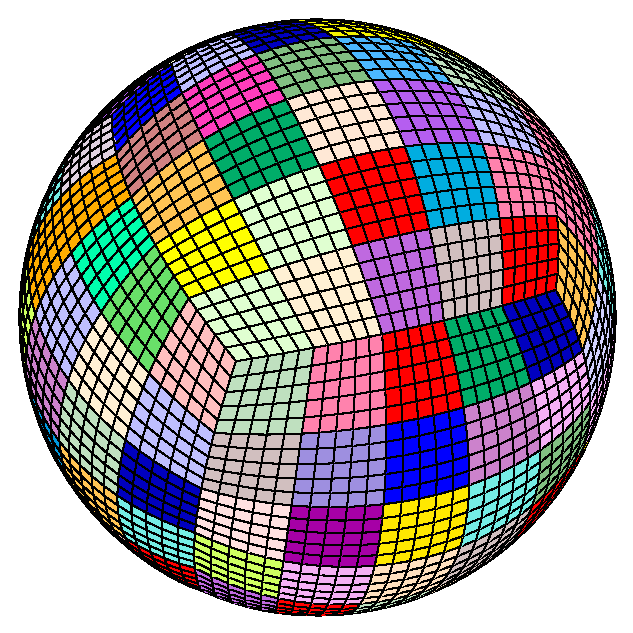
\includegraphics[width=0.45\textwidth]{figures/mpi_slices.eps}
&
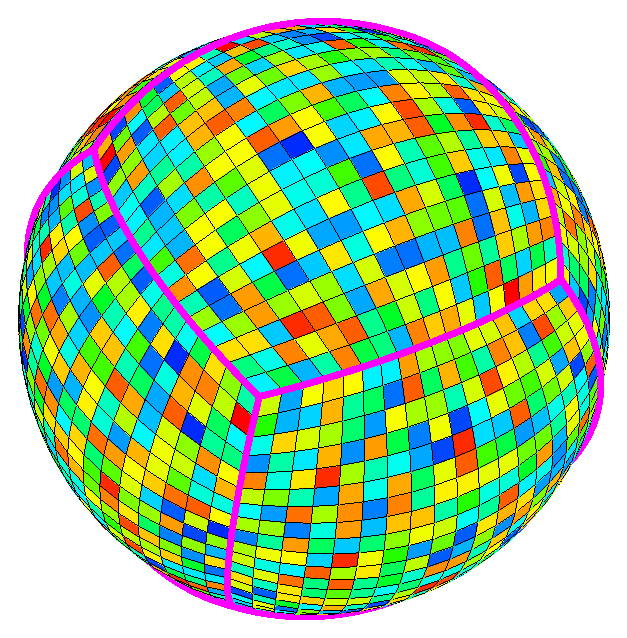
\includegraphics[width=0.45\textwidth]{figures/fullmesh_18.eps}
\end{tabular}
}
\caption{
Each of the 6~chunks that constitutes the cubed sphere is subdivided in terms
of $n^2$~slices of elements, where $n\ge1$ is a positive integer,
for a total of $6\times n^2$ slices (and therefore processors).
The figure on the left shows a mesh that is divided in terms of
$6\times5^2=150$ slices as indicated by the various colors.
In this cartoon,
each slice contains $5\times5=25$ spectral-elements at the Earth's surface.
The figure on the right shows a mesh that is divided over
$6\times18^2=1944$ processors as indicated by the various colors.
Regional simulations are accommodated by using only 1, 2 or 3 chunks of the
cubed sphere.
}
\label{figure:mpi_slices}
\end{figure}
To run the mesher for a global simulation,
the following parameters need to be
set in the \texttt{Par\_file}:
\begin{description}
\item[$\nchunks$] Must be set to 6 for global simulations.
\item[\texttt{ANGULAR\_WIDTH\_XI\_IN\_DEGREES}] Not needed for a global simulation.
(See section~\ref{section:regional} for regional simulations.)
\item[\texttt{ANGULAR\_WIDTH\_ETA\_IN\_DEGREES}] Not needed for a global simulation.
(See section~\ref{section:regional} for regional simulations.)
\item[\texttt{CENTER\_LATITUDE\_IN\_DEGREES}] Not needed for a global simulation.
(See section~\ref{section:regional} for regional simulations.)
\item[\texttt{CENTER\_LONGITUDE\_IN\_DEGREES}] Not needed for a global simulation.
(See section~\ref{section:regional} for regional simulations.)
\item[\texttt{GAMMA\_ROTATION\_AZIMUTH}] Not needed for a global simulation.
(See section~\ref{section:regional} for regional simulations.)
\item[$\nexxi$] The number of spectral-elements along one side of a
chunk in the cubed sphere (see Figure~\ref{figure:mpi_slices}); this
number \textit{must} be 16~$\times$~a multiple of $\nprocxi$ defined below.
We do not recommend using $\nexxi$ less than 64 because
the curvature of the Earth cannot be honored if one uses too few elements.
Furthermore, smaller values of $\nexxi$ are likely to result in spectral
elements with a negative Jacobian, in which case the mesher will exit with
an error message.
Table~\ref{table:nex} summarizes various suitable choices for
$\nexxi$ and the related values of $\nprocxi$.
Based upon benchmarks against semi-analytical
normal-mode synthetic seismograms,
\cite{KoTr02a,KoTr02b} determined that an $\nexxi=240$ run is accurate to
a shortest period of 18~s.
Therefore,
since accuracy is determined by the number of grid points per shortest
wavelength,
for any particular value of $\nexxi$ the simulation will be accurate
to a shortest period determined by
\begin{equation}
\mbox{shortest period (s)} = (240/\nexxi)\times 18.
\label{eq:shortest_period}
\end{equation}
The number of grid points in each orthogonal direction of the
reference element, i.e., the number of Gauss-Lobatto-Legendre points,
is determined by \texttt{NGLLX} in the \texttt{constants.h} file.
In the globel we use $\mbox{\texttt{NGLLX}}=5$, for a total of $5^3=125$
points per elements.
\item[$\nexeta$] For global simulations $\nexeta$
must be set to the same value as $\nexxi$.
\item[$\nprocxi$] The number of processors or slices along one
chunk of the cubed sphere (see Figure~\ref{figure:mpi_slices});
we must have $\nexxi=16\times c\times \nprocxi$, where
$c\ge1$ is a positive integer.
See table~\ref{table:nex} for various suitable choices.
\item[$\nproceta$] For global simulations $\nproceta$
must be set to the same value as $\nprocxi$.
\item[\texttt{MODEL}] Must be set to one of the following:
\begin{description}
\item[\texttt{isotropic\_prem}] Isotropic version of the spherically symmetric
Preliminary Reference Earth Model (PREM) \cite{DzAn81}.
\item[\texttt{transversely\_isotropic\_prem}] Transversely
isotropic version of PREM.
\item[\texttt{iasp91}] Spherically symmetric isotropic IASP91 model \cite{KeEn91}.
\toall{Make sure this gets modified in the code.}
\item[\texttt{ak135}] Spherically symmetric isotropic AK135 model \cite{KeEnBu95}.
\toall{Make sure AK135 gets added to the code.}
\item[\texttt{3D\_isotropic}] By default,
the code uses 3D mantle model S20RTS \cite{RiVaWo99}
and 3D crustal model Crust2.0 \cite{BaLaMa00}.
Note that S20RTS uses transversely isotropic PREM as a background model,
and that we use the PREM radial attenuation model when
\texttt{ATTENUATION} is incorporated.
See section~\ref{section:changingmodels} for a discussion on
how to change 3D models.
\toall{Make sure this gets modified from s20rts in the code.}
\item[\texttt{3D\_anisotropic}]
See section~\ref{section:changingmodels} for a discussion on
how to specify your own 3D anisotropic model.
\toall{Make sure this gets modified from Min\_Chen in the code.}
\item[\texttt{3D\_attenuation}]
See section~\ref{section:changingmodels} for a discussion on
how to specify your own 3D attenuation model.
\toall{Make sure this gets modified from Brian\_Savage in the code.}
\end{description}
\item[\texttt{OCEANS}] Set to \texttt{.true.} if the effect of the oceans
on seismic wave propagation should be incorporated based upon the
approximate treatment discussed in \cite{KoTr02b}. This approximation
is accurate at periods of roughly 20~s and longer. At shorter periods the
effect of water phases/reverberations is not taken into account,
even when the flag is on.
This feature is inexpensive from a numerical perspective, both in terms of
memory requirements and CPU time.
\item[\texttt{ELLIPTICITY}] Set to \texttt{.true.} if the mesh should make the
Earth model elliptical in shape according to Clairaut's equation \cite{DaTr98}.
This feature adds no cost to the simulation.
\item[\texttt{TOPOGRAPHY}] Set to \texttt{.true.} if topgraphy and
bathymetry should be incorporated based upon model ETOPO5 \cite{Etopo5}.
This feature adds no cost to the simulation.
\item[\texttt{GRAVITY}] Set to \texttt{.true.} if self-gravitation
should be incorporated in the Cowling approximation \cite{KoTr02b,DaTr98}.
Turning this feature on is relatively inexpensive, both from the perspective
of memory requirements as well as in terms of speed.
\item[\texttt{ROTATION}] Set to \texttt{.true.} if the Coriolis effect should
be incorporated. Turning this feature on is relatively cheap numerically.
\item[\texttt{ATTENUATION}] Set to \texttt{.true.} if attenuation
should be incorporated. Turning this feature on increases the memory
requirements significantly, and is numerically fairly expensive. Of course for
realistic simulations this flag should be turned on.
See \cite{KoTr99,KoTr02a} for a discussion on the implementation of attenuation
based upon standard linear solids.
\item[\texttt{ABSORBING\_CONDITIONS}] Set to \texttt{.false.} for global
simulations. See section~\ref{section:regional} for regional simulations.
\item[\texttt{RECORD\_LENGTH\_IN\_MINUTES}] Choose the desired
record length of the synthetic seismograms (in minutes). This controls the
length of the numerical simulation, i.e., twice the record length requires
twice as much CPU time. This feature is not used at the time of meshing but
is required for the solver, i.e., you may change this parameter after running
the mesher.
\item[\texttt{MOVIE\_SURFACE}] Set to \texttt{.false.}, unless you want to
create a movie of seismic wave propagation on the Earth's surface.
Turning this option on generates large output files.
See section \ref{section:movies} for a discussion on the generation of
movies.
This feature is not used at the time of meshing but
is relevant for the solver.
\item[\texttt{MOVIE\_VOLUME}] Set to \texttt{.false.}, unless you want to
create a movie of seismic wave propagation in the Earth's interior.
Turning this option on generates huge output files.
See section \ref{section:movies} for a discussion on the generation of
movies.
This feature is not used at the time of meshing but
is relevant for the solver.
\item[\texttt{NTSTEP\_BETWEEN\_FRAMES}] Determines the number of timesteps
between movie frames. Typically you want to save a snapshot every 100
timesteps. The smaller you make this number the more output will be generated!
See section \ref{section:movies} for a discussion on the generation of
movies.
This feature is not used at the time of meshing but
is relevant for the solver.
\item[\texttt{SAVE\_AVS\_DX\_MESH\_FILES}] Set this flag to \texttt{.true.}
to save AVS (\texttt{www.avs.com}), OpenDX (\texttt{www.opendx.org}),
or ParaView (\texttt{www.paraview.org})
mesh files for subsequent viewing.
Turning the flag on generates large (distributed)
files in the \texttt{LOCAL\_PATH} directory.
See section~\ref{section:meshgraphics} for a discussion
of mesh viewing features.
\item[\texttt{NUMBER\_OF\_RUNS}] On machines with a run-time limit, a simulation
may need to be completed in stages. This option allows you to select the number of
stages in which the simulation will be completed (1, 2 or 3). Choose 1 for
a run without restart files.
This feature is not used at the time of meshing but
is required for the solver.
At the end of the first or second stage of a multi-stage simulation,
large files are written to the file system to save the current
state of the simulation. This state is read back from the file system
at the beginning of the next stage of the multi-stage run.
Reading and writing the states can be very time consuming depending on
the nature of the network and the file system.
\item[\texttt{NUMBER\_OF\_THIS\_RUN}] If you choose to perform the run in
stages, you need to tell the solver what stage run to perform.
This feature is not used at the time of meshing but
is required for the solver.
\item[\texttt{LOCAL\_PATH}]
Directory in which the databases generated by the mesher will be written.
Generally one uses a directory on the local disk of the compute nodes,
although on some machines these databases are written on a parallel (global)
file system
(see also the earlier discussion of the
\texttt{LOCAL\_PATH\_IS\_ALSO\_GLOBAL} flag in section~\ref{section:gettingstarted}).
The mesher generates the necessary databases in parallel,
one set for each of the $6\times\nprocxi^2$ slices that constitutes
the mesh (see Figure~\ref{figure:mpi_slices}).
After the mesher finishes, you can login to one of the compute nodes and
view the contents of the \texttt{LOCAL\_PATH} directory to see the (many) files
generated by the mesher.
\item[\texttt{MACHINE\_FILE}] Set this parameter to the MPI machine
file in the \texttt{SPECFEM3D\_GLOBE\_V3.6} directory.
This file tells MPI which compute nodes to use in the simulation.
The file must have a number of entries (one entry per line) equal
to the number of processors needed for the run.
A sample \texttt{MACHINE\_FILE} is provided in the file
\texttt{mymachines}.
See section~\ref{section:scheduler} for information about running
the code on a system with a scheduler, e.g., LSF.
\item[\texttt{NTSTEP\_BETWEEN\_OUTPUT\_INFO}] This parameter specifies
the interval at which basic information about a run is written to the file system
(\texttt{timestamp*} files in the \texttt{OUTPUT\_FILES} directory).
If you have access to a fast machine, set \texttt{NTSTEP\_BETWEEN\_OUTPUT\_INFO}
to a relatively high value (e.g., at least 100, or even 1000 or more)
to avoid writing output text files too often.
This feature is not used at the time of meshing.
\item[\texttt{NTSTEP\_BETWEEN\_OUTPUT\_SEISMOS}] This parameter specifies
the interval at synthetic seismograms are written in the
\texttt{LOCAL\_PATH} directory. If a run crashes, you may still
find usable (but shorter than requested)
seismograms in this directory.
On a fast machine set \texttt{NTSTEP\_BETWEEN\_OUTPUT\_SEISMOS}
to a relatively high value to avoid writing to the seismograms too often.
This feature is not used at the time of meshing.
\item[\texttt{RECEIVERS\_CAN\_BE\_BURIED}] This flags accommodates
stations with instruments that are buried, i.e., the solver will calculate
seismograms at the burial depth specified in the \texttt{STATIONS} file.
This feature is not used at the time of meshing.
\item[\texttt{PRINT\_SOURCE\_TIME\_FUNCTION}] Turn this flag on
to print information about the source time function in
the file \texttt{OUTPUT\_FILES/plot\_source\_time\_function.txt}.
This feature is not used at the time of meshing.
\end{description}

\begin{table}[t]
\begin{tabular}{|c|c|rrrrr|} \hline
\multicolumn{1}{|c|}{$\nprocxi$} & \multicolumn{1}{|c|}{processors} &
\multicolumn{5}{|c|}{$\nexxi$ (shortest period in seconds)} \\ \hline
1 & 6 & 64 (68) & 80 (54) & 96 (45) & 112 (39) & 128 (34) \\
2 & 24 & 64 (68) & 96 (45) & 128 (34) & 160 (27) & 192 (23) \\
3 & 54 & 96 (45) & 144 (30) & 192 (23) & 112 (39) & 240 (18) \\
4 & 96 & 64 (68) & 128 (34) & 192 (23) & 256 (17) & 320 (14) \\
5 & 150 & 80 (54) & 160 (27) & 240 (18) & 320 (14) & 400 (11) \\
6 & 216 & 96 (45) & 192 (23) & 288 (15) & 384 (11) & 480 (9) \\
7 & 294 & 112 (39) & 224 (19) & 336 (13) & 448 (10) & 560 (8) \\
8 & 384 & 128 (34) & 256 (17) & 384 (11) & 512 (9) & 640 (7) \\
9 & 486 & 144 (30) & 288 (15) & 432 (10) & 576 (8) & 720 (6) \\
10 & 600 & 160 (27) & 320 (14) & 480 (9) & 640 (7) & 800 (5) \\
11 & 726 & 176 (25) & 352 (12) & 528 (9) & 704 (6) & 880 (5) \\
12 & 864 & 192 (23) & 384 (11) & 576 (8) & 768 (6) & 960 (5) \\
13 & 1014 & 208 (21) & 416 (10) & 624 (7) & 832 (5) & 1040 (4) \\
14 & 1176 & 224 (19) & 448 (10) & 672 (6) & 896 (5) & 1120 (4) \\
15 & 1350 & 240 (18) & 480 (9) & 720 (6) & 960 (5) & 1200 (4) \\
16 & 1536 & 256 (17) & 512 (9) & 768 (6) & 1024 (4) & 1280 (3) \\
17 & 1734 & 272 (16) & 544 (8) & 816 (5) & 1088 (4) & 1360 (3) \\
18 & 1944 & 288 (15) & 576 (8) & 864 (5) & 1152 (4) & 1440 (3) \\
19 & 2166 & 304 (14) & 608 (7) & 912 (5) & 1216 (4) & 1520 (3) \\
20 & 2400 & 320 (14) & 640 (7) & 960 (5) & 1280 (3) & 1600 (3) \\
21 & 2646 & 336 (13) & 672 (6) & 1008 (4) & 1344 (3) & 1680 (3) \\
22 & 2904 & 352 (12) & 704 (6) & 1056 (4) & 1408 (3) & 1760 (2) \\
23 & 3174 & 368 (12) & 736 (6) & 1104 (4) & 1472 (3) & 1840 (2) \\
24 & 3456 & 384 (11) & 768 (6) & 1152 (4) & 1536 (3) & 1920 (2) \\
25 & 3750 & 400 (11) & 800 (5) & 1200 (4) & 1600 (3) & 2000 (2) \\
26 & 4056 & 416 (10) & 832 (5.2) & 1248 (3.5) & 1664 (2.6) & 2080 (2.1) \\
\hline
\end{tabular}
\caption{
Sample choices for $\nexxi$ given $\nprocxi$ based upon the
relationship $\nexxi=16\times c\times \nprocxi$, where the integer $c\ge1$.
The number of MPI slices, i.e., the total `number of required processors,
is $6\times \nexxi^2$, as illustrated in Figure~\ref{figure:mpi_slices}.
The number in parenthesis is the shortest period at which the
global simulation is accurate.
This shortest period is determine based upon
equation (\ref{eq:shortest_period}).
For regional simulations the shortest period of the
simulation may be determined based upon
(\ref{eq:shortest_period_regional}).
The largest run to date involved 4056 processors of the Earth Simulator
and $\nexxi=1248$; this simulation was accurate to a shortest period of 3.5~s.
}
\label{table:nex}
\end{table}
Now that you have set the appropriate parameters in the \texttt{Par\_file}
and have compiled the mesher, you are ready to launch it! This is most
easily accomplished based upon the \texttt{go\_mesher} script.
When you run on a PC cluster,
the script assumes that the nodes are named n001, n002, etc.
If this is not the case, change the \texttt{tr -d 'n'} line in the script.
You may also need to edit the last command at the end of the script that invokes the
\texttt{mpirun} command.

Mesher output is provided in the \texttt{OUTPUT\_FILES} directory in
\texttt{output\_mesher.txt};
this file provides lots of details about the mesh that was generated.
Alternatively, output can be directed to the screen instead
by uncommenting a line in constants.h:
\begin{verbatim}
       ! uncomment this to write messages to the screen
       ! integer, parameter :: IMAIN = ISTANDARD_OUTPUT )
\end{verbatim}

Another file generated by the mesher is
the header file \texttt{OUTPUT\_FILES/values\_from\_mesher.h}.
This file specifies a number of constants and flags needed by the solver.
These values are passed statically to the solver for reasons of speed.
Some useful statistics about the mesh are also
provided in this file.

For a given model, set of nodes, and set of parameters in \texttt{Par\_file},
one only needs to run the mesher once and for all, even if one wants
to run several simulations with different sources and/or receivers
(the source and receiver information is used in the solver only).

\subsection{Checking the MPI Buffers (Optional)}

\todimitri{You may want to expand on this section a bit more.}
The mesher writes MPI communication tables in the \texttt{OUTPUT\_FILES}
subdirectory in the files \texttt{addressing.txt},
\texttt{list\_messages\_corners.txt} and \texttt{list\_messages\_faces.txt}.
Use the four serial codes \texttt{check\_buffers\_1D.f90},
\texttt{check\_buffers\_2D.f90}, \texttt{check\_buffers\_faces\_chunks.f90}
and \texttt{check\_buffers\_corners\_chunks.f90} to check all the MPI buffers
generated by the mesher (e.g., type
`\texttt{make check\_buffers\_1D}' and then `\texttt{xcheck\_buffers\_1D}').

\subsection{Checking the Mesh Quality (Optional)}
\label{section:quality}

\todimitri{You may want to expand on this section a bit more.}
The quality of the mesh may be inspected based upon the serial code
\texttt{check\_mesh\_quality\_AVS\_DX.f90}.
Type `\texttt{make check\_mesh\_quality\_AVS\_DX}' and then use
`\texttt{xcheck\_mesh\_quality\_AVS\_DX}' to generate an AVS output file
(\texttt{AVS\_meshquality.inp} in AVS UCD format)
or an OpenDX output file (\texttt{DX\_meshquality.dx})
that can be used to investigate mesh quality, e.g., skewness of elements
and a Gnuplot histogram (\texttt{mesh\_quality\_histogram.txt}) that can
be plotted with gnuplot (type `\texttt{gnuplot plot\_mesh\_quality\_histogram.gnu}').
Once you are brave enough to start designing your own meshes, this tool is
useful for viewing your creations. You are striving for meshes with
elements with `cube-like' dimensions, e.g., the mesh should
contain no very elongated or skewed elements.

\section{Running the Solver \texttt{xspecfem3D}}
\label{section:solver}

Now that you have successfully run the mesher, you are ready to compile the solver.
For reasons of speed, the solver uses static memory allocation. Therefore it
needs to be recompiled (type `\texttt{make clean}' and `\texttt{make specfem3D}')
every time one reruns the mesher.
To compile the solver one needs a file generated by the mesher in
the directory \texttt{OUTPUT\_FILES} called
\texttt{values\_from\_mesher.h},
which contains parameters describing the static size of the arrays
as well as the setting of certain flags, e.g., `\texttt{GRAVITY\_VAL}'.

The solver needs three input files in the \texttt{DATA} directory to run:
the \texttt{Par\_file} which was discussed in detail in
section~\ref{section:mesher},
the earthquake source parameter file \texttt{CMTSOLUTION}, and the
stations file \texttt{STATIONS}.
Most parameters in the \texttt{Par\_file} should be set
prior to running the mesher. Only the following parameters may be changed
after running the mesher: the record length \texttt{RECORD\_LENGTH\_IN\_MINUTES},
the movie control parameters \texttt{MOVIE\_SURFACE}, \texttt{MOVIE\_VOLUME},
and \texttt{NTSTEPS\_BETWEEN\_FRAMES}, the multi-stage simulation
parameters \texttt{NUMBER\_OF\_RUNS} and \texttt{NUMBER\_OF\_THIS\_RUN},
the output information parameters \texttt{NTSTEP\_BETWEEN\_OUTPUT\_INFO}
and \texttt{NTSTEP\_BETWEEN\_OUTPUT\_SEISMOS},
and the \texttt{RECEIVERS\_CAN\_BE\_BURIED} and
\texttt{PRINT\_SOURCE\_TIME\_FUNCTION} flags.
Any other change to the \texttt{Par\_file} implies rerunning both
the mesher and the solver.

For any particular earthquake,
the \texttt{CMTSOLUTION} file that represents the point source may be
obtained directly from the Harvard Centroid-Moment Tensor
(CMT) web page  (\texttt{www.seismology.harvard.edu}).
It looks like this:
\begin{verbatim}
PDE 1999 11 26 13 21 15.60 -16.4200  168.2100  33.0 6.4 7.3 VANUATU ISLANDS
event name:     112699G
time shift:     11.2000
half duration:  10.0000
latitude:      -16.0800
longitude:     168.3100
depth:          15.0000
Mrr:       1.310000e+27
Mtt:       1.200000e+26
Mpp:      -1.420000e+27
Mrt:       4.600000e+26
Mrp:       8.200000e+26
Mtp:      -2.000000e+26
\end{verbatim}
The \texttt{CMTSOLUTION} should be edited in the following way:
\begin{itemize}
\item Set the \texttt{time shift} parameter equal to $0.0$
(the solver will not run otherwise.)
The time shift parameter would simply apply an overall DC shift to the
synthetics, something that can be done in the post-processing.
\item For most simulations we recommend setting the source
half-duration parameter \texttt{half duration} equal to zero,
which corresponds to simulating a step source-time function,
i.e., a moment-rate function that is a delta function.
If \texttt{half duration} is not set to zero,
the code will use a Gaussian (very nearly triangular)
source-time function with half-width \texttt{half duration}.
We prefer to run the solver with \texttt{half duration}
set to zero and convolve the resulting synthetic seismograms after the fact,
because this way it's easy to use a variety of source-time functions.
\cite{KoTr02a} determined that the noise generated in the simulation by
using a step source time function may be safely filtered out afterward
based upon a convolution with the desired source time function
and/or low-pass filtering.
Use the serial code \texttt{convolve\_source\_timefunction.f90} and the script
\texttt{convolve\_source\_timefunction.csh} for this purpose.
Set the parameter \texttt{hdur} in \texttt{convolve\_source\_timefunction.csh}
to the desired half-duration and
type `\texttt{make convolve\_source\_timefunction}' to compile the code.
\end{itemize}
Centroid latitude and longitude should be provided in geographical coordinates.
The code converts these coordinates to geocentric coordinates~\cite{DaTr98}.
Of course you may provide your own source representations by
designing your own \texttt{CMTSOLUTION} file.
Just make sure that the resulting file adheres to the Harvard CMT
conventions (see appendix~\ref{appendix:coordinates}).
The implementation of finite (kinematic) sources is discussed
in section~\ref{section:finitesources}.

The solver can calculate seismograms at any number of stations for
basically the same numerical cost, so the user is encouraged to
include as many stations as conceivably useful in the \texttt{STATIONS} file,
which looks like this:
\begin{verbatim}
755
MCK   AK   63.7323  -148.9349  618.0    0.0
CTAO  AS  -20.0882   146.2545  357.0    0.0
KONO  AS   59.6491     9.5982  216.0    0.0
MAJO  AS   36.5409   138.2083  431.0    0.0
ZOBO  AS  -16.2700   -68.1250 4450.0    0.0
ASBS  AZ   33.6208  -116.4664 1400.0    0.0
BZN   AZ   33.4915  -116.6670 1301.0    0.0
CRY   AZ   33.5654  -116.7373 1128.0    0.0
.
.
.
\end{verbatim}
The first line in this file should indicate the number of stations listed
in the file.
Each subsequent line represents one station in the following format:
\begin{verbatim}
Station Network Latitude (degrees) Longitude (degrees) Elevation (m) burial (m)
\end{verbatim}
Station latitude and longitude should be provided in geographical coordinates.
The width of the station label should be 32 characters or less,
and the network code should be 8 characters wide.

Solver output is provided in the \texttt{OUTPUT\_FILES} directory in
the \texttt{output\_solver.txt} file.
Output can be directed to the screen instead by uncommenting a line in constants.h:
\begin{verbatim}
       ! uncomment this to write messages to the screen
       ! integer, parameter :: IMAIN = ISTANDARD_OUTPUT )
\end{verbatim}
On PC clusters the seismogram files are generally written to the
local disks (the path \texttt{LOCAL\_PATH} in the \texttt{Par\_file})
and need to be gathered at the end of the simulation.

While the solver is running, its progress may be tracked by monitoring the
`\texttt{timestamp*}' files in the \texttt{OUTPUT\_FILES} directory.
These tiny files look something like this:
\begin{verbatim}
 Time step #           200
 Time:    0.6956667      minutes
 Elapsed time in seconds =     252.6748970000000
 Elapsed time in hh:mm:ss =    0 h 04 m 12 s
 Mean elapsed time per time step in seconds =     1.263374485000000
 Max norm displacement vector U in solid in all slices (m) =       1.9325
 Max non-dimensional potential Ufluid in fluid in all slices =    1.1058885E-22
\end{verbatim}
They tell you the \texttt{Mean elapsed time per time step in seconds},
which may be used to assess performance on various machines,
as well as the \texttt{Max norm displacement vector U in solid in all slices (m)}
and
\texttt{Max non-dimensional potential Ufluid in fluid in all slices}.
If something is wrong with the model, the mesh, or the source, you will
see the code become unstable through exponentionally growing
values of the displacement and fluid potential with time.
You can control the rate at which the timestamp files are written
based upon the parameter \texttt{NTSTEP\_BETWEEN\_OUTPUT\_INFO}
in the \texttt{Par\_file}.

Having set the \texttt{Par\_file} parameters, and having
provided the \texttt{CMTSOLUTION} and \texttt{STATIONS} files,
you are now ready to launch the solver!
This is most
easily accomplished based upon the \texttt{go\_solver} script.
You may need to edit the last command at the end of the script that invokes the
\texttt{mpirun} command.
The \texttt{runall} script compiles and runs both mesher and solver
in sequence. This is a safe approach that ensures using the
correct combination of mesher output and solver input.

It is important to realize that the CPU and memory requirements of the
solver are closely tied to choices about attenuation
(\texttt{ATTENUATION}), self-gravitation (\texttt{GRAVITY}),
and the nature of the model (i.e., isotropic models are cheaper than
anisotropic models).
We encourage you to run a variety of simulations with various
flags turned on or of to develop a sense for what is involved.

For the same model, one can rerun the solver for different events by simply
changing the CMTSOLUTION file, or for different stations by changing the
STATIONS file. There is no need to rerun the mesher.
Of course it is best to include as many stations as possible, since this
does not add to the cost of the simulation.

\section{Regional Simulations}
\label{section:regional}

The code has the option of running in 1, 2, 3 or 6 chunk mode.
The 1, 2 or 3 chunk options may be used for higher
resolution regional simulations.
A 1 chunk mesh may have lateral dimensions other than the
customary $90^\circ$ per chunk, which can further increase the resolution
of the mesh, and thus reduce the shortest period in the synthetics.
A disadvantage of regional simulations is that one needs to use
absorbing boundary conditions on the side and bottom edges of the model.
Figure~\ref{figure:one_chunk} shows an example of a 1 chunk mesh centered
on the Fiji-Tonga area.
\begin{figure}
\centerline{
\begin{tabular}{cc}
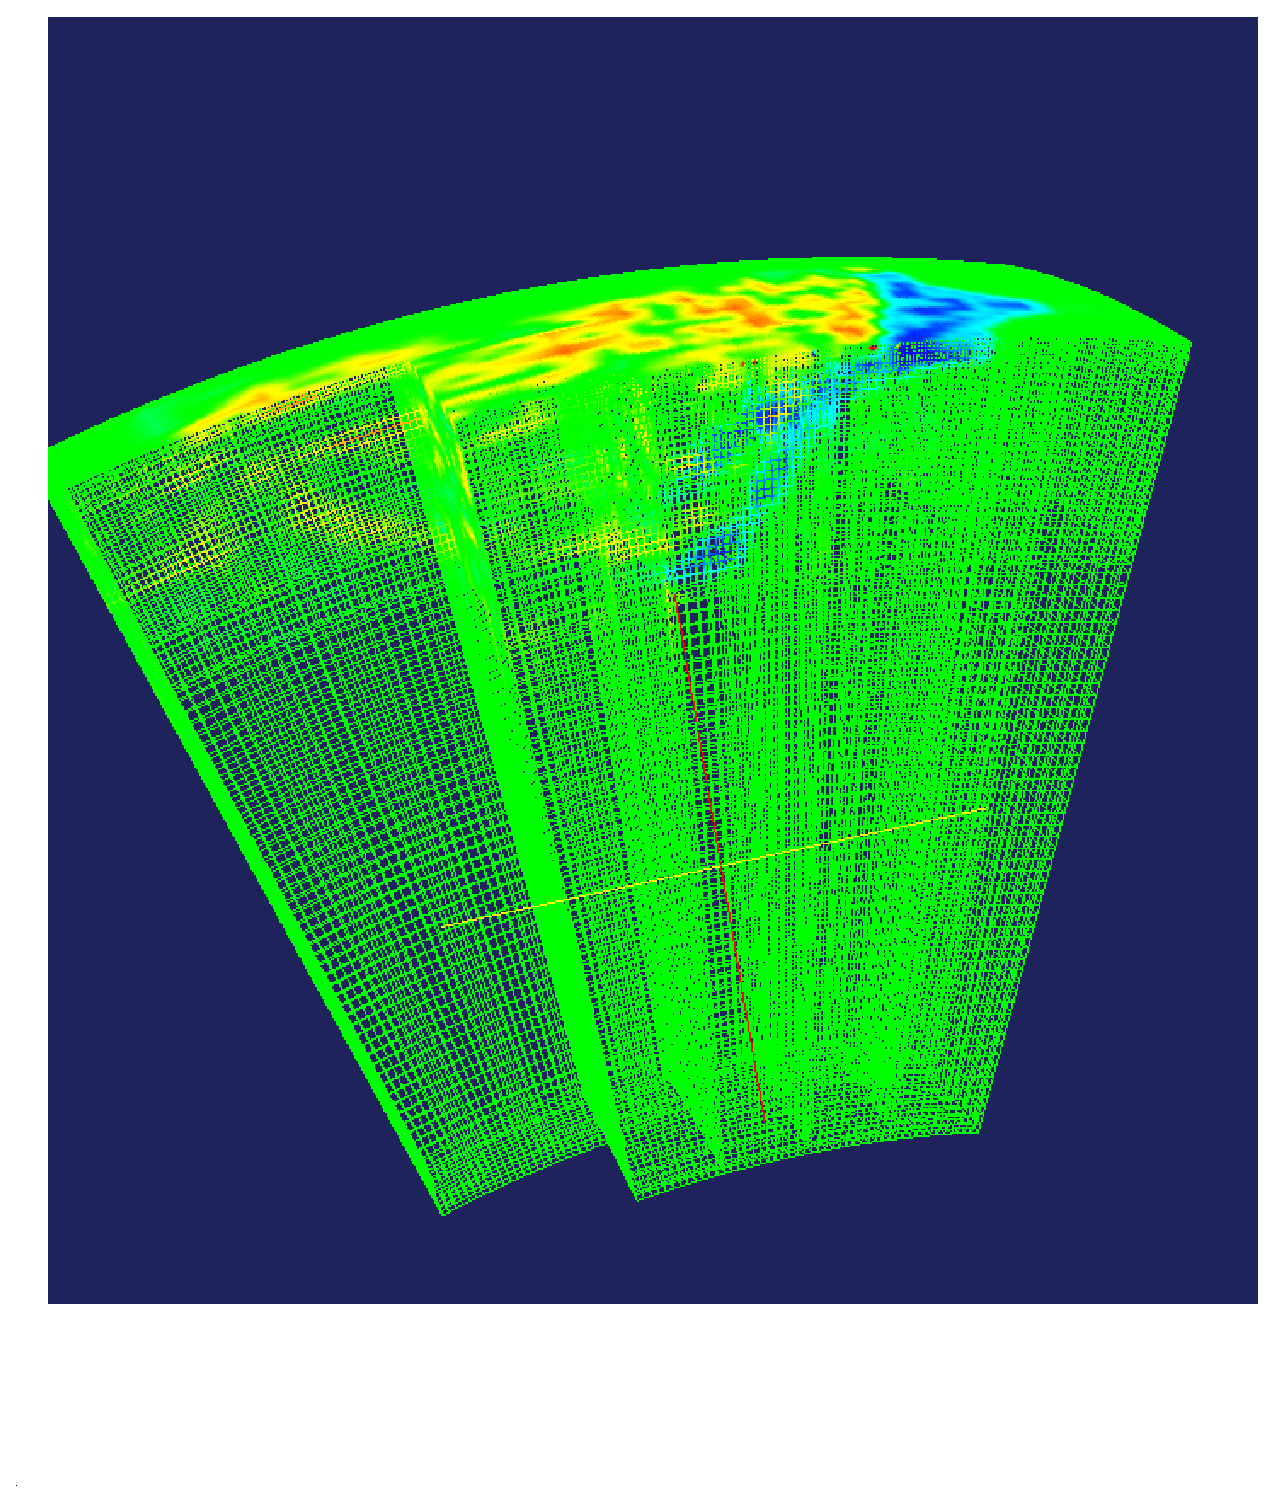
\includegraphics[width=0.45\textwidth]{figures/all_vp_grid.eps}
&
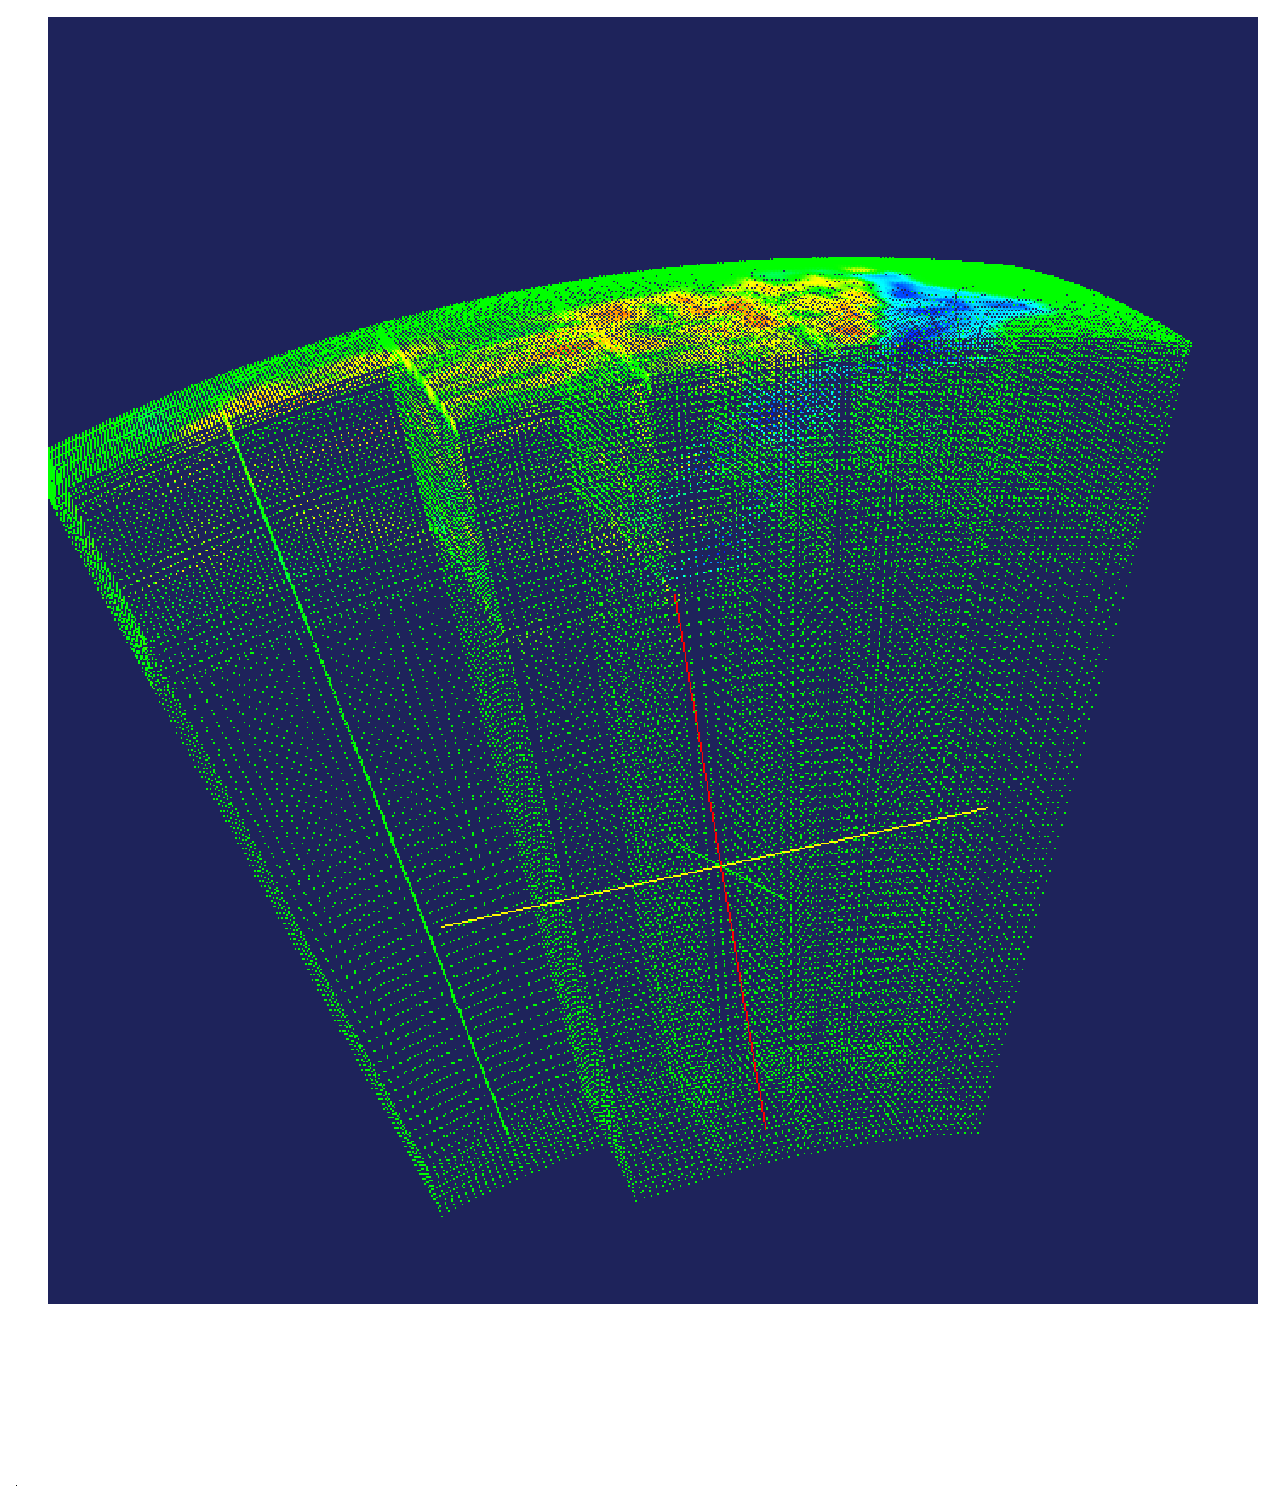
\includegraphics[width=0.45\textwidth]{figures/all_vp_points.eps}
\end{tabular}
}
\caption{
Lateral variations in relative compressional wave speed in the Fiji-Tonga
area. Left: spectral-element mesh. Right: GLL points.
}
\end{figure}

\subsection{1 Chunk Simulations}

\tobrian{Please double check this section carefully!}
For a 1 chunk regional simulation the following parameters need to be set
in the \texttt{Par\_file}:
\begin{description}
\item[$\nchunks$] Must be set to 1
\item[\texttt{ANGULAR\_WIDTH\_XI\_IN\_DEGREES}] Denotes the width of
one side of the chunk (degrees).
\item[\texttt{ANGULAR\_WIDTH\_ETA\_IN\_DEGREES}] Denotes the width of
the second side of the chunk (degrees).
Note that this value may be different from
\texttt{ANGULAR\_WIDTH\_XI\_IN\_DEGREES}.
\item[\texttt{CENTER\_LATITUDE\_IN\_DEGREES}] Defines the latitude of the
center of the chunk (degrees).
\item[\texttt{CENTER\_LONGITUDE\_IN\_DEGREES}] Defines the longitude of the
center of the chunk (degrees).
\item[\texttt{GAMMA\_ROTATION\_AZIMUTH}] Defines the rotation angle of the
chunk about its center measured clockwise from due North (degrees).
\tobrian{Verify this convention.}.
\item[$\nexxi$] The number of spectral-elements along the
$\xi$ side of the chunk.
This number \textit{must} be 16~$\times$~a multiple of $\nprocxi$ defined below.
For a $90^\circ$ chunk,
we do not recommend using $\nexxi$ less than 64 because
the curvature of the Earth cannot be honored if one uses too few elements.
\item[$\nexeta$] The number of spectral-elements along the
$\eta$ side of the chunk.
This number \textit{must} be 16~$\times$~a multiple of $\nproceta$ defined below.
Note that to get elements that are close to square on the Earth's surface the ratios
$(\texttt{ANGULAR\_WIDTH\_XI\_IN\_DEGREES}/\nexxi)$
and
$(\texttt{ANGULAR\_WIDTH\_ETA\_IN\_DEGREES}/\nexeta)$
should be similar.
\item[$\nprocxi$] The number of processors or slices along the $\xi$ side of the
chunk.
To accommodate the mesh doubling layers,
we must have $\nexxi=16\times c\times \nprocxi$, where
$c\ge1$ is a positive integer.
See table~\ref{table:nex} for various suitable choices.
\item[$\nproceta$] The number of processors or slices along the $\eta$ side of the
chunk;
we must have $\nexeta=16\times c\times \nproceta$, where
$c\ge1$ is a positive integer.
$\nprocxi$ and $\nproceta$ must be equal when $\nchunks = 6$ or
$\nchunks = 3$. The option of having different values for $\nprocxi$
and $\nproceta$ is available only for regional simulations
when $\nchunks = 1$ (1/6th of the sphere)
or $\nchunks = 2$.
\item[\texttt{ABSORBING\_CONDITIONS}] Set to \texttt{.true.} for regional
simulations.
Note that the absorbing boundary conditions are never perfect, and in particular
surface wave may partially reflect off the artificial boundaries.
Note also that certain arrivals, e.g., PKIKPPKIKP, will be missing from
the synthetics.
\end{description}
When the width of the chunk is different from~$90^\circ$, the radial
distribution of the elements needs to be adjusted as well to maintain
spectral elements that are as cube-like as possible. The code attempts
to do this, but be sure to view the mesh with your favorite graphics
package to make sure that the elements are well behaved.
We also recommend that you use the serial code
\texttt{check\_mesh\_quality\_AVS\_DX.f90} to check the quality of the mesh
(see section~\ref{section:quality}). Remember: a high-quality mesh
is paramount for accurate simulations.

The shortest period at which a regional simulation is accurate may be determined based
upon the relation
\begin{equation}
\mbox{shortest period (s)} = (240/\nexxi)\times
(\texttt{ANGULAR\_WIDTH\_XI\_IN\_DEGREES}/90)\times 18.
\label{eq:shortest_period_regional}
\end{equation}

\subsection{2 or 3 Chunk Simulations}

\todimitri{Please provide a description of how the 2 and 3 chunk options may be used,
what the \texttt{ANGULAR\_WIDTH\_XI\_IN\_DEGREES}, etc., parameters mean
in this case, and perhaps figures illustrating 2 and 3 chunk meshes.}

\section{Adjoint Simulations}

\toqinya{Please provide a step-by-step description of how the adjoint code
is used.}

\subsection{Adjoint sources}

\tovalaqinya{Please explain in this section how adjoint sources may be used,
e.g., for kinematic source studies.}

\subsection{Finite-Frequency Kernels}

\toqinya{Include figure for illustration.}

\section{Graphics}

\toqinya{Please add to this discussion about graphics for meshes, kernels, etc.
Also update the text to reflect the ParaView capabilities.}

\subsection{Meshes}
\label{section:meshgraphics}

Use the serial code \texttt{combine\_AVS\_DX.f90}
(type `\texttt{make combine\_AVS\_DX}' and then
`\texttt{xcombine\_AVS\_DX}') to generate AVS (\texttt{www.avs.com}) output files
(in AVS UCD format) or OpenDX (\texttt{www.opendx.org}) output files showing the mesh,
the MPI partition (slices), the $\nchunks$ chunks, the
source and receiver location, etc.
Use the AVS UCD files \texttt{AVS\_continent\_boundaries.inp} and
\texttt{AVS\_plate\_boundaries.inp} or the OpenDX files
\texttt{DX\_continent\_boundaries.dx} and \texttt{DX\_plate\_boundaries.dx}
for reference.

\subsection{Movies}
\label{section:movies}

\tovalaqinya{Please elaborate on this discussion.}

To make a surface or volume movie of the simulation,
set parameters
\texttt{MOVIE\_SURFACE}, \texttt{MOVIE\_VOLUME}, and \texttt{NTSTEP\_BETWEEN\_FRAMES}
in the \texttt{Par\_file}.
Turning on the movie flags, in particular  \texttt{MOVIE\_VOLUME}, produces
large output files.
We typically save the vertical component of the velocity field.
The look of a movie is determined by the half duration of the source.
The half-duration should be large enough such that the movie does
not contain frequencies that are not resolved by the mesh, i.e., it should
not contain numerical noise.
This may be accomplished by \tovalaqinya{please fill in}.

After you have run \texttt{xspecfem3D} with the movie flags turned on,
use \texttt{create\_movie\_AVS\_DX.f90} (type `\texttt{make create\_movie\_AVS\_DX}')
to create a movie of surface displacement (radial component) or of the entire 3D wave
field. The movie can be saved in OpenDX, AVS, or ParaView format.
Set parameters
\texttt{MOVIE\_SURFACE}, \texttt{MOVIE\_VOLUME}, and \texttt{NTSTEP\_BETWEEN\_FRAMES}
in the \texttt{Par\_file}.

\subsection{Finite-Frequency Kernels}

\toqinya{Please explain in this section how finite-frequency kernels
may be constructed.}

\section{Running through a Scheduler}
\label{section:scheduler}

The code is usually run on large parallel machines, often PC clusters,
most of which use schedulers: queuing or batch management systems to manage
the running of jobs from a large number of users.
The following considerations need to be taken into account when running on
a system that uses a scheduler:
\begin{itemize}
\item The processors/nodes to be used for each run are assigned dynamically
by the scheduler, based on availability.
Therefore, in order for the mesher and the solver to have access to the same
mesh files (usually stored on hard drives local to the nodes on which the
code is run), they must be launched in sequence as a single job.
\item On some systems, the nodes to which running jobs are assigned are
not configured for compilation.
It may, therefore, be necessary to pre-compile both the mesher and the solver.
A small program called \texttt{create\_header\_file.f90}, provided in the
distribution, can be used to directly create
\texttt{OUTPUT\_FILES/values\_from\_mesher.h} using the information in
the \texttt{DATA/Par\_file} without having to run the mesher
(type '\texttt{make create\_header\_file}' to compile it
and '\texttt{xcreate\_header\_file}' to run it).
The solver can now be compiled as before.
\item One feature of schedulers/queuing systems is that they allow
submission of multiple jobs in a ``launch and forget'' mode.
In order to take advantage of this property, care needs to be taken that
output and intermediate files from separate jobs do not overwrite each other,
or otherwise interfere with other running jobs.
\end{itemize}

We describe here in some detail a job submission procedure for the
Caltech 1024-node cluster, CITerra, under the LSF scheduling system.
We consider the submission of a forward simulation using the global
code and the \texttt{s20rts} Earth model.
The two main scripts are \texttt{queue\_forward\_global\_s20rts.sh},
which sets up a launch directory and submits the job to the scheduler,
and \texttt{go\_mesher\_solver\_lsf.bash}, which contains the instructions
that make up the job itself.
These scripts can straight-forwardly be modified and adapted to meet
more specific running needs.
%%
\subsection{\texttt{queue\_forward\_global\_s20rts.sh}}
This script requires the \texttt{SPECFEM3D} code to be pre-compiled as
described above . It is invoked as follows:

\texttt{queue\_forward\_global\_s20rts.sh PATH-TO-SPECFEM3D-CODE
CMTSOLUTION-FILE STATION-FILE [QUEUE-NAME]},

where \texttt{PATH-TO-SPECFEM-CODE} is the path to the directory containing the
compiled version of the \texttt{SPECFEM3D} code,
\texttt{CMTSOLUTION-FILE} is a file containing the source information in
Harvard CMT format (see section~\ref{section:running}, \texttt{STATION-FILE}
is a file containing the list of stations (again see section~\ref{section:running}
for the format), and  \texttt{QUEUE-NAME} is an optional argument specifying
the name of the queue the job is to be submitted to.

The script starts by parsing the input information, setting up the environment,
and if necessary creating the base directory in which the launch directory
for this job will be created:

{\small
\begin{verbatim}
#!/bin/bash

# Parse input
code_dir=$1
cmt_file=$2
station_file=$3
queue="-q normal"
if [ $# -eq 4 ] ; then
  echo "Setting the queue to $4"
  queue="-q $4"
fi

# obtain the full path to the code_dir
here=`pwd`
cd $code_dir
code_dir=`pwd`
cd $here

# Set environment
export IFORT_ROOT=/opt/intel/fc/9.0.026
export MPI_ROOT=/opt/mpichgm-1.2.6..14b..gcc_3.2.3..ifort_9.0.026
. ${IFORT_ROOT}/bin/ifortvars.sh
export PATH=${MPI_ROOT}/bin:${PATH}:/opt/lsfhpc/6.0/linux2.4-glibc2.3-ia32e/bin
export LD_LIBRARY_PATH=${MPI_ROOT}/lib:${LD_LIBRARY_PATH}

# Create the base directory for launching of event runs
event_base=${HOME}/LAUNCH_EVENTS
if [ ! -e $event_base ] ; then
  mkdir -p $event_base
fi

\end{verbatim}}

The next step is to create a uniquely named launch directory, from which the
job will subsequently be submitted to the scheduling system.
This launch directory will need to have copies of all the information needed
for the run.
All the outputs and products from the run will also be collected here.
The \texttt{queue\_} script creates the name of the launch directory from
the earthquake identifier in the \texttt{CMTSOLUTION-FILE},
and from the name of the \texttt{SPECFEM3D} code directory
(which acts as an identifier of the version of the code being run).
Other naming schemes are of course possible.

{\small
\begin{verbatim}

# Construct the name of the launch directory, and create it
event_name=`grep event $cmt_file | awk '{print $NF}'`
code_name=`echo $code_dir | awk -F"/" '{print $NF}'`
event_dir=${event_base}/${event_name}_${code_name}

# If the launch directory already exists, then this may already have
# been run
if [ -d $event_dir ] ; then
  echo "Event dir $event_dir already exists - will not queue job"
  exit 2
fi

# make the directory from which this event simulation will be launched
mkdir -p $event_dir

\end{verbatim}}

Now the script creates a file called \texttt{comments.txt} in the launch
directory, in which all the information relevant to the setup of this run
is recorded.
If a file of the same name is present in the \texttt{SPECFEM3D} code
directory, containing for example a description of changes that were
made to this particular version of the code, then its contents are appended
to this file.

{\small
\begin{verbatim}

# Create a comments file including all the information about this run
echo `date` > ${event_dir}/comments.txt
echo "-----" >> ${event_dir}/comments.txt
echo "Code path : $code_dir" >> ${event_dir}/comments.txt
echo "CMT file  : $cmt_file" >> ${event_dir}/comments.txt
echo "Stations  : $station_file" >> ${event_dir}/comments.txt
echo "-----" >> ${event_dir}/comments.txt
if [ -e ${code_dir}/comments.txt ] ; then
  cat ${code_dir}/comments.txt >> $event_dir/comments.txt
fi
echo "-----" >> ${event_dir}/comments.txt

\end{verbatim}}

The next step is to copy or make symbolic links to the executables and
other files necessary for the code to run.
Executables and model directories are symbolically linked to, the other
files are copied.
Scripts necessary for other set-up steps, and for seismogram retrieval and
post-run clean-up are also copied into the launch directory at this time.

{\small
\begin{verbatim}
# link the executables from the code directory
ln -s ${code_dir}/xmeshfem3D ${event_dir}/xmeshfem3D
ln -s ${code_dir}/xspecfem3D ${event_dir}/xspecfem3D

# copy / link the relevant DATA files
mkdir ${event_dir}/DATA
ln -s ${code_dir}/DATA/crust2.0 ${event_dir}/DATA/crust2.0
ln -s ${code_dir}/DATA/s20rts ${event_dir}/DATA/s20rts
ln -s ${code_dir}/DATA/topo_bathy ${event_dir}/DATA/topo_bathy
cp ${code_dir}/DATA/Par_file ${event_dir}/DATA/Par_file
cp ${station_file} ${event_dir}/DATA/STATIONS
cp ${cmt_file} ${event_dir}/DATA/CMTSOLUTION


# copy scripts
cp ${HOME}/bin/go_mesher_solver_lsf_global.bash ${event_dir}
cp ${HOME}/bin/remap_lsf_machines.pl ${event_dir}
cp ${HOME}/bin/collect_seismo_lsf_multi.pl ${event_dir}
cp ${HOME}/bin/cleanmulti.pl ${event_dir}
\end{verbatim}}

The final pre-submission step is to compute the number of processors :

{\small
\begin{verbatim}
# compute total number of processors needed
NPROC_XI=`grep NPROC_XI ${event_dir}/DATA/Par_file | cut -c 34- `
NPROC_ETA=`grep NPROC_ETA ${event_dir}/DATA/Par_file | cut -c 34- `
NCHUNKS=`grep NCHUNKS ${event_dir}/DATA/Par_file | cut -c 34- `
numprocs=$(( $NCHUNKS * $NPROC_XI * NPROC_ETA ))
\end{verbatim}
}

The final step is to \texttt{cd} to the launch directory and submit
the job using the lsf job submission command, \texttt{bsub}
(type '\texttt{man bsub}' on CITerra to learn about the \texttt{bsub} command).
The job sequence itself is detailed in the \texttt{go\_mesher\_solver\_lsf.bash}
script described in the following sub-section.

{\small
\begin{verbatim}
echo "Submitting job from : $event_dir"
cd ${event_dir}
echo "bsub $queue -n $numprocs < go_mesher_solver_lsf_global.bash"
bsub $queue -n $numprocs < go_mesher_solver_lsf_global.bash

\end{verbatim}}

%%
\subsection{\texttt{go\_mesher\_solver\_lsf.bash}}

This script describes the job itself, including set-up steps that can only
be done once the scheduler has assigned the job a job id and a set of
compute nodes, the \texttt{mpirun.lsf} commands used to run the mesher and
the solver, and calls to scripts that collect the output seismograms from
the compute nodes and perform clean-up operations.

The first portion of the script directs the scheduler to save its own
output and the output from \texttt{stdout} into \texttt{OUTPUT\_FILES/\%J.o},
where \texttt{\%J} is a short-hand for the job-id; it also tells the scheduler
which version of mpich to use (\texttt{mpich\_gm}) and how to name this
job (\texttt{go\_mesher\_solver\_lsf}).

{\small
\begin{verbatim}
#!/bin/bash
#BSUB -o OUTPUT_FILES/%J.o
#BSUB -a mpich_gm
#BSUB -J go_mesher_solver_lsf
\end{verbatim}}

The next portion creates the \texttt{OUTPUT\_FILES} directory and creates
a list of the nodes allocated to this job by echoing the value of a
dynamically set environment variable \texttt{LSB\_MCPU\_HOSTS} and parsing the
output into a one-column list using the perl script \texttt{remap\_lsf\_machines.pl}.
It then creates a set of scratch directories on these nodes to be used as
the \texttt{LOCAL\_PATH} for temporary storage of the mesh files.
These scratch directories are named using the job-id in order to ensure
they are unique to this job (the job-id is given by the dynamically set
environment variable \texttt{LSB\_JOBID}): \\
\texttt{/state/partition1/scratch/\${USER}/DATABASES\_MPI.\$LSB\_JOBID}.
The scratch directories are created using \texttt{shmux}, a shell multiplexor
that can execute the same commands on many hosts in parallel.
\texttt{shmux} is available from \texttt{http://web.taranis.org/shmux/}.
The script then changes the \texttt{LOCAL\_PATH} parameter in
\texttt{DATA/Par\_file} to the job-specific scratch directory name.

{\small
\begin{verbatim}
if [ -z $USER ]; then
  echo "could not run go_mesher_solver_lsf.bash as no USER env is set"
  exit 2
fi

BASEMPIDIR=/state/partition1/scratch/${USER}/DATABASES_MPI

# script to run the mesher

# read DATA/Par_file to get information about the run

rm -r -f OUTPUT_FILES
mkdir OUTPUT_FILES

echo "$LSB_MCPU_HOSTS" > OUTPUT_FILES/lsf_machines
echo "$LSB_JOBID" > OUTPUT_FILES/jobid

./remap_lsf_machines.pl OUTPUT_FILES/lsf_machines >OUTPUT_FILES/machines

# now just make the dir (cleanup should be done afterwards after collect seismos,
# otherwise  we clean up a nother runs seismos)
shmux -M50 -Sall -c "mkdir -p $BASEMPIDIR.$LSB_JOBID" - < OUTPUT_FILES/machines \
>/dev/null

# now modify the Par_file to have the proper path specific to this job id
# this ASSUMES that the Par_file just has a vanilla LOCAL_PATH line
sed -e "s:^LOCAL_PATH .*:LOCAL_PATH                      =  $BASEMPIDIR.$LSB_JOBID:" \
< DATA/Par_file > DATA/Par_file.tmp
mv DATA/Par_file.tmp DATA/Par_file

\end{verbatim}}

The script then parses \texttt{DATA/Par\_file} and outputs to
\texttt{stdout} information about the \texttt{LOCAL\_PATH} and the number
of processors to be used for this run.
This information will be saved in the \texttt{OUTPUT\_FILES/\%J.o} file.

{\small
\begin{verbatim}

# compute total number of nodes needed
NPROC_XI=`grep NPROC_XI DATA/Par_file | cut -c 34- `
NPROC_ETA=`grep NPROC_ETA DATA/Par_file | cut -c 34- `
NCHUNKS=`grep NCHUNKS ${event_dir}/DATA/Par_file | cut -c 34- `

# total number of nodes is the product of the values read
numnodes=$(( $NCHUNKS * $NPROC_XI * NPROC_ETA ))

# output this information to stdout
echo NPROC_XI = $NPROC_XI
echo NPROC_ETA = $NPROC_ETA
echo " "
echo starting MPI mesher on $numnodes processors
echo " "
echo starting run in current directory $PWD
echo " "
echo mesh files will be saved in directory $my_local_path on the nodes
echo " "
\end{verbatim}}

The next portion of the script launches the mesher and then the solver
using \texttt{mpirun.lsf}:

{\small
\begin{verbatim}
#### use this on LSF
mpirun.lsf --gm-no-shmem --gm-copy-env $PWD/xmeshfem3D
mpirun.lsf --gm-no-shmem --gm-copy-env $PWD/xspecfem3D
\end{verbatim}}

The final portion of the script collects the seismograms and performs
clean-up on the nodes, using the perl scripts
\texttt{collect\_seismo\_lsf\_multi.pl} and \texttt{cleanmulti.pl}:

{\small
\begin{verbatim}
# collect seismograms and clean up
here=$PWD
mkdir SEMD
cd SEMD
../collect_seismo_lsf_multi.pl ../OUTPUT_FILES/lsf_machines ../DATA/Par_file
cd $here
./cleanmulti.pl OUTPUT_FILES/machines DATA/Par_file
\end{verbatim}
}

\section{Kinematic Ruptures}
\label{section:finitesources}

\tovala{Please elaborate on kinematic rupture simulations. Explain how the half
duration and timeshift in the CMTSOLUTION file are used, etc. A cartoon
might be helpful.}

To simulate a kinematic rupture, i.e., a finite-source event,
represented in terms of $N_\mathrm{sources}$,
provide a \texttt{CMTSOLUTION} file that has $N_\mathrm{sources}$ entries,
one for each subevent (i.e., concatenate $N_\mathrm{sources}$ CMTSOLUTION files
to a single CMTSOLUTION file).
At least one entry must have a zero \texttt{time shift},
and all the other entries must have non-negative \texttt{time shift}. Each subevent
can have its own half duration, latitude, longitude, depth, and moment tensor.

\section{Changing the Model}
\label{section:changingmodels}

In this section we explain how to change the crustal, mantle, and
inner core models. These changes involve contributing specific
subroutines that replace existing subroutines in the
\texttt{SPECFEM3D\_GLOBE} package.

\subsection{Changing the Crustal Model}

The 3D crustal model Crust2.0 \cite{BaLaMa00} is superimposed on
to the mesh by the subroutine \texttt{crustal\_model.f90}.
To accomplish this,
the flag \texttt{CRUSTAL}, set in the subroutine
\texttt{read\_parameter\_file.f90},
is used to signal a 3D crustal model.
When this flag is set to \texttt{.true.},
the crust on top of the 1D reference model (PREM, IASP91, or AK135) is
removed and replaced by extending the mantle.
The 3D crustal model is subsequently overprinted on to the crust-less
1D reference model.
The call to the 3D crustal routine is of the form
\begin{verbatim}
call crustal_model(lat,lon,r,vp,vs,rho,moho,found_crust)
\end{verbatim}
Input to this routine are:
\begin{description}
\item[\texttt{lat}] Latitude in degrees.
\item[\texttt{lon}] Longitude in degrees.
\item[\texttt{r}] Non-dimensionalized radius ($0<\texttt{r}<1$).
\end{description}
Output from the routine are:
\begin{description}
\item[\texttt{vp}] Non-dimensionalized compressional wave speed
at location (\texttt{lat},\texttt{lon},\texttt{r}).
\item[\texttt{vs}] Non-dimensionalized shear wave speed.
\item[\texttt{rho}] Non-dimensionalized density.
\item[\texttt{moho}] Non-dimensionalized Moho depth.
\item[\texttt{found\_crust}] Logical that is set to \texttt{.true.} only
if crust exists at location (\texttt{lat},\texttt{lon},\texttt{r}),
i.e., \texttt{.false.} for radii \texttt{r} in the mantle.
This flags determines whether or not a particular location is in the crust
and, if so, what parameters to assign to the mesh at this location.
\end{description}
All output needs to be non-dimensionalized according to the convention
summarized in appendix~\ref{appendix:conventions}.
You can replace this subroutine by your own routine
\textit{provided you do not change the call structure of the routine},
i.e., the new routine should take exactly the same input and
produce the required, properly non-dimensionalized output.

Part of the file \texttt{crustal\_model.f90} is the
subroutine \texttt{read\_crustal\_model}.
The call to this routine takes no arguments and is used to once-and-for-all
read in the databases related to Crust2.0. When you choose to replace
the file \texttt{crustal\_model.f90} with your own implementation you
\textit{must} provide a \texttt{read\_crustal\_model} routine,
even if it does nothing.
Model constants read by the routine \texttt{read\_crustal\_model}
are passed to the subroutine \texttt{read\_crustal\_model} through
the module \texttt{crustal\_model\_constants},
and model variables are passed via the module
\texttt{crustal\_model\_variables}.
An alternative crustal model should use the same constructs.

\subsection{Changing the Mantle Model}

This section discusses how to change isotropic and anisotropic
3D mantle models. Usually such changes go hand-in-hand with
changing the 3D crustal model.

\subsubsection{Isotropic Models}

The 3D mantle model S20RTS \cite{RiVaWo99} is superimposed on to
the mantle mesh by the subroutine \texttt{mantle\_model.f90}.
The call to this subroutine is of the form
\begin{verbatim}
call mantle_model(radius,theta,phi,dvs,dvp,drho)
\end{verbatim}
Input to this routine are:
\begin{description}
\item[\texttt{radius}] Non-dimensionalized radius
($\texttt{RCMB/R\_EARTH}<\texttt{r}<\texttt{RMOHO/R\_EARTH}$;
for a given 1D reference model,
the constants \texttt{RCMB} and \texttt{RMOHO} are set in the
\texttt{read\_parameter\_file.f90} file).
The code expects the isotropic mantle model to be defined between the Moho
(with radius \texttt{RMOHO} in m) and the core-mantle boundary (CMB;
radius \texttt{RCMB} in m) of a 1D reference model.
When a 3D crustal model is superimposed, as will usually
be the case, the 3D mantle model is stretched to fill any potential
gap between the radius of the Moho in the 1D reference model
and the Moho in the 3D crustal model.
Thus, when the Moho in the 3D crustal model is shallower than the Moho in
the reference model, e.g., typically below the oceans,
the mantle model is extended to fill this gap.
\item[\texttt{theta}] Colatitude in radians.
\item[\texttt{phi}] Longitude in radians.
\end{description}
Output from the routine are the following non-dimensional perturbations:
\begin{description}
\item[\texttt{dvs}] Relative shear-wave speed perturbations $\delta\beta/\beta$
at location (\texttt{radius},\texttt{theta},\texttt{phi}).
\item[\texttt{dvp}] Relative compressional-wave speed perturbations $\delta\alpha/\alpha$.
\item[\texttt{drho}] Relative density perturbations $\delta\rho/\rho$.
\end{description}
You can replace the \texttt{mantle\_model.f90} file by your own version
\textit{provided you do not change the call structure of the routine},
i.e., the new routine should take exactly the same input and
produce the required relative output.

Part of the file \texttt{mantle\_model.f90} is the
subroutine \texttt{read\_mantle\_model}.
The call to this routine takes no arguments and is used to once-and-for-all
read in the databases related to S20RTS. When you choose to replace
the file \texttt{mantle\_model.f90} with your own implementation you
\textit{must} provide a \texttt{read\_mantle\_model} routine,
even if it does nothing.
Model constants read by the routine \texttt{read\_mantle\_model}
are passed to the subroutine \texttt{read\_mantle\_model} through
the module \texttt{three\_d\_mantle\_model\_constants},
and model variables are passed via the module
\texttt{three\_d\_mantle\_model\_variables}.
An alternative mantle model should use the same constructs.

\subsubsection{Anisotropic Models}

3D anisotropic mantle models may be superimposed on the mesh based
upon the subroutine \texttt{anisotropic\_mantle\_model.f90}.
The call to this subroutine is of the form
\begin{verbatim}
call aniso_mantle_model(r,theta,phi,rho, &
    c11,c12,c13,c14,c15,c16,c22,c23,c24,c25,c26, &
    c33,c34,c35,c36,c44,c45,c46,c55,c56,c66)
\end{verbatim}
\tomin{Would you remove the myrank parameter from the call?}
Input to this routine are:
\begin{description}
\item[\texttt{r}] Non-dimensionalized radius
($\texttt{RCMB/R\_EARTH}<\texttt{r}<\texttt{RMOHO/R\_EARTH}$;
for a given 1D reference model,
the constants \texttt{RCMB} and \texttt{RMOHO} are set in the
\texttt{read\_parameter\_file.f90} file).
The code expects the anisotropic mantle model to be defined between the Moho
and the core-mantle boundary (CMB).
When a 3D crustal model is superimposed, as will usually
be the case, the 3D mantle model is stretched to fill any potential
gap between the radius of the Moho in the 1D reference model
and the Moho in the 3D crustal model.
Thus, when the Moho in the 3D crustal model is shallower than the Moho in
the reference model, e.g., typically below the oceans,
the mantle model is extended to fill this gap.
\item[\texttt{theta}] Colatitude in radians.
\item[\texttt{phi}] Longitude in radians.
\end{description}
Output from the routine are the following non-dimensional model parameters:
\begin{description}
\item[\texttt{rho}] Non-dimensionalized density $\rho$.
\item[\texttt{c11}, $\cdots$, \texttt{c66}] 21 non-dimensionalized
anisotropic elastic parameters.
\end{description}
You can replace the \texttt{anisotropic\_mantle\_model.f90} file by your own version
\textit{provided you do not change the call structure of the routine},
i.e., the new routine should take exactly the same input and
produce the required relative output.
Part of the file \texttt{anisotropic\_mantle\_model.f90} is the
subroutine \texttt{read\_aniso\_mantle\_model}.
The call to this routine takes no arguments and is used to once-and-for-all
read in the static databases related to the anisotropic model.
When you choose to replace
the file \texttt{anisotropic\_mantle\_model.f90} with your own implementation you
\textit{must} provide a \texttt{read\_aniso\_mantle\_model} routine,
even if it does nothing.
Model constants read by the routine \texttt{read\_mantle\_model}
are passed through
the module \texttt{aniso\_mantle\_model\_constants},
and model variables are passed via the module
\texttt{aniso\_mantle\_model\_variables}.
An alternative anisotropic mantle model should use the same constructs.

Rotation of the anisotropic tensor elements from one coordinate
system to another
coordinate system may be accomplished based upon the subroutine
\texttt{rotate\_aniso\_tensor}.
Use of this routine requires understanding the coordinate
system used in \texttt{SPECFEM3D\_GLOBE},
as discussed in appendix~\ref{appendix:coordinates}.

%\subsection{Changing the Inner Core Model}
%
\subsection{Anelastic Models}

3D anelastic (attenuation) models may be superimposed on the mesh based
upon the subroutine
\texttt{attenuation\_model}.  The call to this routine is as such
\begin{verbatim}
call attenuation_model(myrank, latitude, longitude, radius, Qmu, tau_s,
tau_e, T_c_source, &

RICB,RCMB,RTOPDDOUBLEPRIME,R600,R670,R220,R771,R400,R80)
\end{verbatim}
Input to this routine are:
\begin{description}
\item[\texttt{myrank}] Current pocessor rank.
\item[\texttt{latitude}] Latitude in degrees ($ -90 <= \theta <= 90$).
\item[\texttt{longitude}] Longitude in degrees ($-180 <= \phi <= 180 $).
\item[\texttt{radius}] radius in km ($ 0 <= r <= r_\mathrm{earth}$).
\item[\texttt{R*}] radii of particular layers in meters.
\end{description}
Output to this routine are:
\begin{description}
\item[\texttt{Qmu}] Shear wave quality factor ($ 0 < Q_\mu < 5000 $).
\item[\texttt{tau\_s}] dimension(N\_SLS) Stress relaxation time.  These
values only depend on the
curent period range of interest.  They should be constant across all
calls to this subroutine.
\item[\texttt{tau\_e}] dimension(N\_SLS) Strain relaxation time.  These
values depend on the period
range of interest and on the value of the quality factor (\texttt{Qmu}) for that
specific point.
\item[\texttt{T\_c\_source}] Effective time width of the source, should
be constant across all calls
to te subroutine.
\end{description}

If run without modification, the subroutine \texttt{attenuation\_model}
will implement the PREM attneuation
structure.  If you would like to implement your own attenuation model,
you need to modify your model
using the \texttt{attenuation\_model} subroutine as a guide or write
your own.  It is not enough to just set
the value of Qmu to the edesired value, the internal solver variables
tau\_s, tau\_e, and T\_c\_source must be determined.
Conversion from Qmu to the internal solver variables is done by calling
the subroutine \texttt{attenuation\_conversion}
as such
\begin{verbatim}
call attenuation_conversion(myrank, Qmu, T_c_source, tau_s, tau_e)
\end{verbatim}
with the input being myrank and Qmu and the output as T\_c\_source, tau\_s
and tau\_e.

\tojeroen{I think variables myrank and the RICB, R* need to be removed
from the function calls}

\section{Bug reports and suggestions of improvements}

To report bugs or suggest improvements to the code, please send an email
to Jeroen Tromp (\texttt{jtromp AT caltech.edu}) and/or use our online
bug tracking system at \texttt{http://www.geodynamics.org/roundup}.

\section*{Notes \& Acknowledgments}

The Gauss-Lobatto subroutines in \texttt{gll\_library.f90} are based in part on
software libraries from M.I.T., Department of Mechanical Engineering.
The non-structured global numbering software was provided by Paul F. Fischer.
Subroutines from ``Numerical Recipes: The Art of Scientific Computing''
by W.H.\ Press et al., Cambridge University Press, are used in
\texttt{numerical\_recipes.f90}. The user must acquire an official
Numerical Recipes license to run them.
OpenDX is open-source based on IBM Data Explorer, \texttt{www.opendx.org},
AVS is a trademark of Advanced Visualization Systems, \texttt{www.avs.com},
and ParaView is an open-source visualization
platform available via \texttt{www.paraview.com}.
The following individuals contributed to this manual:
Min Chen, Vala Hjorleifsdottir, Dimitri Komatitsch, Qinya Liu,
Alessia Maggi, Brian Savage, and Jeroen Tromp.
Please e-mail your feedback, comments, and suggestions to
Jeroen Tromp (\texttt{jtromp AT caltech.edu}).

%%%%%%%%% BIBLIOGRAPHY %%%%%%%%%%%%%%%%%%%%%%%

%\clearpage
\bibliography{bibliography}

%%%%%%%%% APPENDICES %%%%%%%%%%%%%%%%%%%%%%%

\appendix

\section{Synthetic Seismogram Timing Convention}

\tovalaqinya{Here we should show a picture of a time series, illustrating what
zero is, how the Gaussian source time function works, how the time
shift is implemented, etc.}

\section{Memory Requirements}
\tovalabrian{Please check and elaborate on this section. If possible, add a couple
of figures illustrating memory needs.}

A typical SPECFEM3D\_GLOBE simulation involves roughly 60~GB of distributed
memory and a few tens of processors. For example,
a PC cluster with 27 dual processor nodes, each with 3~GB of memory,
enables one to calculate fully 3D synthetic seismograms with
a 1~hour record length accurate at periods of 18~s and longer in roughly
20~hours.
The largest simulation to date involved 4056 processors and 7.8~TB
of distributed memory on the Earth Simulator at
Japan Agency for Marine-Earth Science and Technology (JAMSTEC)
\cite{KoTsChTr03,TsKoChTr03}; this simulation enabled us to reach a
shortest period of 3.5~s.

The SPECFEM3D\_GLOBE memory requirements are proportional to
$\nexxi\times \nexeta\times R$,
where $\nexxi$ and $\nexeta$ are the number of elements along each side of a
chunk, and $R$ is a measure of the number of elements in the radial
direction (which are set automatically in the read\_parameter\_file.f90 file).
Assume that $\nexxi=\nexeta=16\times c\times n$,
where $n=\nprocxi=\nproceta$ and $c$ is an integer.
The factor of 16 is there to accommodate the three doublings in the mesh
below the Moho, at the 670~km discontinuity, and just above the ICB.
Now $\nexxi\times \nexeta\times R = (16\times c\times n)^2\times R$.

To estimate the constant of proportionality we can scale to a run
that has $\nexxi=\nexeta=240$ (i.e., $n=5$, $c=3$), in single precision,
with all the fancy stuff (gravity, rotation, attenuation, etc.) turned on.
This run needs around 60~GB of RAM.
Thus we need $\mbox{60~GB}/(240\times 240\times 6\times R_{240})=174/R_{240}$ kB
of memory per element,
where $R_{240}$ is a measure of the number of elements in the radial
direction for an $\nexxi=\nexeta=240$ run.
As a result, proportionally for a different run:
$\mbox{memory needed}=174 \mbox{kB}\times 6\times (16\times c\times n)^2 \times R/R_{240}$.
The memory available is given by $6\times n^2\times\mbox{memory/processor}$
(for a run on 6 chunks).
To satisfy the starting equation we need that:
$174\mbox{kB}\times 6\times (16\times c\times n)^2 \times R/R_{240}
< 6\times n^2\times \mbox{memory/processor}$
or:
\begin{equation}
\mbox{memory/processor} > c^2 \times R/R_{240}\times \mbox{45~MB}.
\end{equation}
Note that this is independent of the number of processors.
Now, if the memory/processor is large, we can increase $c$, and thus $\nexxi$ and $\nexeta$
to a large number and run a high resolution run.
However, the number of elements per processor
(basically $c^2 \times R/R_{240}$) goes up,
increasing the computing time as $c^2\times R/R_{240}$.
Figure~\ref{figure:R} illustrates the behavior of
$R/R_{240}$ as a function of $\nexxi$.

\section{Reference Frame Convention}
\label{appendix:coordinates}

The code uses the following convention for the Cartesian reference frame:
\begin{itemize}
\item the $x$ axis points East
\item the $y$ axis points North
\item the $z$ axis points up
\end{itemize}
Note that this convention is different from both the \cite{AkRi80} convention
and the Harvard Centroid-Moment Tensor (CMT) convention.
The Aki \& Richards convention is
\begin{itemize}
\item the $x$ axis points North
\item the $y$ axis points East
\item the $z$ axis points down
\end{itemize}
and that the Harvard CMT convention is
\begin{itemize}
\item the $x$ axis points South
\item the $y$ axis points East
\item the $z$ axis points up
\end{itemize}

\section{Non-Dimensionalization Conventions}
\label{appendix:conventions}

All physical parameters used by the code are non-dimensionalized according
to the conventions summarized in table~\ref{table:conventions}.
\begin{table}[ht]
\begin{tabular}{|c|c|} \hline
quantity (units) & non-dimensionalized with \\ \hline
distance (m) & \texttt{R\_EARTH} \\
time (s) & $\sqrt{\texttt{PI}\times\texttt{GRAV}\times\texttt{RHOAV}}$ \\
density (kg/m${}^3$) & \texttt{RHOAV} \\ \hline
\end{tabular}
\caption{
Non-dimensionalization employed by the code. The constants
\texttt{R\_EARTH} (the radius of the Earth),
\texttt{PI} (the number $\pi$), \texttt{GRAV} (the universal gravitational constant),
and \texttt{RHOAV} (the Earth's average density)
are set in the \texttt{constants.h} file.
}
\label{table:conventions}
\end{table}

\end{document}
